\section{Features}

Over all the challege was to understand what makes a vine popular. And for that the there was a need to explore correlations of all the possible abstract midlevel features made available to us because of the rapid development in the fields of Deep machine learning. The main important contribution of machine learning is the ability of computationally extracting abstract higher level representations, which vaguely represent human perception. 

\subsection{Low level Aesthetic Features}:
There are some well known computationally evaluatable aesthetic features which have been recognized as heuristics for good photography. Examples include Rule of thirds, Sharp Pixel proportion, Contrast, Simplicity, Left- Right symmetry etc \cite{yeh2010personalized}. The parameters basically compute perceptual features of an image based on well know heurestic rules set by photographers. Some of the detailed references of the features we use are 

\subsubsection{Contrast}
Contrast is basically dissmilarity between pixel(colour) values in a picture. It is a good aesthetic measure to understand how the photographer or creator of a visualc content has used the range of colour values to his advantage. This measure does not always reflect the aesthetic  quality of an image, but with other features like sharp pixel proportion, can be a good approximation. For the sake of our study, we use Weber contrast, which is defined as 
\begin{equation}
F_\textit{weber} = \sum_{x = width}\sum_{y = height} \frac{I(x,y) - I_\textit{average}}{I_\textit{average}} 
\end{equation}


\subsubsection{Simplicity}
Simplicty of composition of a photograph is a distinguishible factor that directly correlates with professionalism of the creator \cite{ke2006design}. We use simplicity definition as defined in \cite{yeh2010personalized} to calculate the ROI segment simplicity and Luo simplicity \cite{luo2008photo}

\subsubsection{Rule of Thirds}
This feature deals with compositional aspects of a photograph. Several papers including \cite{yeh2010personalized} study this feature and hence we use this as one of our aesthetic features. This feature basically calculates if the object of interest is placed in one of the imaginary intersection of lines drawn at approximate onethird of the horizontal and vertical postions. This is a well known aesthetic guideline for photographers.

\subsubsection{Sharp Pixel Proportion}
Out of focus or blurry photographs are generally not considered aesthetically pleasing. In this feature we measure the proportion of sharp pixels compared to total pixels. To do so we have to transform the image from intensity domain to frequency domain, and then count the total number of pixels which surpass the shapness criterion. We choose the criterion of sharpness in frequency domain to be 2 from \cite{yeh2010personalized}. The processing of the images was done using a tool called OpenIMAJ \cite{Hare:2011:OIJ:2072298.2072421}

\subsubsection{L-R Balance}
Difference in intensity of pixels between two sections of an image is also a good measure of aesthetic quality. In non-ideal lighting conditions, images and videos tend to be over exposed in one part and correctly exposed in other. This is generally a sign of amature creator. To capture this we compare the distribution of intensities of pixels in the left and right side of the image. The distance between the two distributions is measured using Chi-squared distance.

\subsubsection{Naturalness}
This is a very heuristic property if an image that tries to gauge the degree of correspondence of images to the human perception. We first convert the image from RGB to HSL colour space which is proved to be closer to human perception of colours. We then group pixels using a heuristic rule that chooses pixels corresponding to natural objects like skin, grass, sky, water etc. This is done by choosing pixels which have L \begin{math} \in \end{math} [20 , 80] and S > 0.1. The final naturalness score is calulated by finding the weighted average of all the groups of pixels. \cite{predictingPintrest}

\subsubsection{Colourfulness}
This is measure of an image's difference against a pure Gray image. It calculated as specified in \cite{yeh2010personalized}


\subsection{ Presence of Faces }
One important aspect of micro videos is the presence of user as an actor in the video. When you look at viral vine videos, most videos seem to have a lead actor performing a skit. The hypothesis here was that vine has become a social media network, where actors have gained prominence and become a reason for popularity. So we did a small experiment, where we sample one image every second from all the videos collected. Then we calculate the percentage of frames across each video which contained at least one face in it. We use the well tested Viola Jones dectector for frontal and profile face detection. \cite{viola2004robust}. When we plot the CDF of these percentages for popular against unpopular videos we see considerably higher population of popular videos to have high number of face image percentage \ref{fig:Face_CDF}.


\subsection{Frame Sentiments}

The crawled vine dataset was sampled and processed using the Multi Lingual sentibank detectors \cite{jou2015visual} which expresses visual sentiment of video feames on the scale of 1 to 5, 1 being negative and 5 being positive sentiments. To make use of this framework we randomly select about 12000 videos from the collection of 80k plus videos having both popular and unpopular vines. Then we sample these videos for frames twice every second. This creates a time series of video frames which could be now fed into the deep neural network for estimation of sentiments. These sentiments are basically vectors of length 12, (vine videos can be at most 6 seconds long) and there are 12000 such vectors. We can now do some statistical analysis on this N x 12 matrix


\subsection{Audio Features}
Along with aesthetic and perceptual sentiment features, audio is a big part of the Vine clip. We decided to use features that resonate more with the perceptual side of the analysis than the low level. We use 6 features that signify \cite{redi20146} perceptual attributes like loudness, rhythemical features, roughness etc. We extract these perceptual features using open source tools and incorporate them in the list of features we use for analysis \cite{lartillot2007matlab} \cite{laurier2009exploring}. 

\subsection{Social Features}
To incorporate the effects of the social visibility for a post, the follower count and the past post count of the user who posts a particular video is used along with all the percieved features. 

\begin{figure}[!htb]
\centering
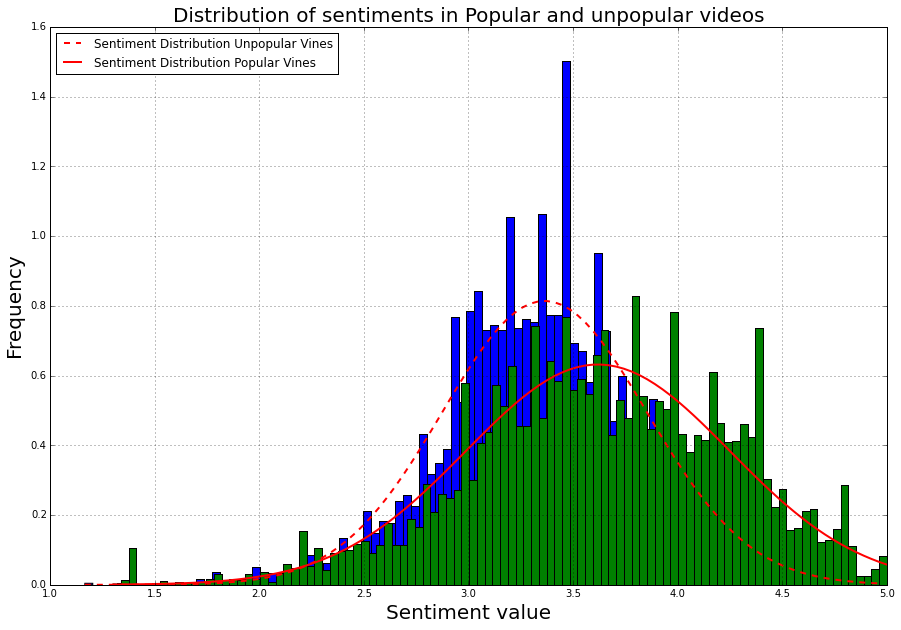
\includegraphics[width=\columnwidth]{plots/DistributionSentiments}
\caption{\textsl{ Distribution of sentiment values for Popular and unpopular videos. The distributions follow a Gaussian like curve, but Popular videos tend to have more positive sentiments than Unpopular }}
\label{fig:Senti_distribution}
\end{figure}


\begin{table*}[t]
  \centering
	\resizebox{2\columnwidth}{!}{
	\begin{tabular}{ | l | l | l | p{5cm} |}
  	 \hline
  	 \textbf{Feature Name} & \textbf{Dimensions} & \textbf{Description} \\
  	\hline
  	\hline
   	Mean Sentiment  & 1 & Mean of sentiments detected using sentibank \cite{pappas2016multilingual}\\
   	\hline
   	\hline
   	 Contrast  & 3 & Frame contrast calculated using Webber, color and RMS techniques \\
   	 \hline
   	 Simplicity & 2 & Image simplicity calculated by two methods \cite{yeh2010personalized} \\
   	 \hline
   	 Naturalness & 1 & A measure of "Naturalness" of a frame \\
   	 \hline
   	 Colourfulness & 1 & A measure of colourfullness that describes the deviation from a pure gray image \\
   	 \hline
   	 Hue Stats & 2 & Hue mean and variance which signifies the range of pure colours present in the image \\
   	 \hline
   	 LR balance & 1 & The Chi squared distance between the histogram of Left and Right side of image pixels.\\
   	 \hline
   	  Object Saliency & 2 & Measure of prominance given to salient objects. Includes Rule of thirds and ROI proportion \\
   	 \hline
   	  Image brightness & 3 & Features signify brightness of the image. Includes average brightness, saturation  and saturation variance\\
   	 \hline
   	 Image sharpness & 2 & Features signify how sharp an image is. Includes sharpness variance and sharp pixel proportion \\
   	\hline 
   	\hline
   	Audio Rhytmical Features & 2 & Onset rate and zero crossing rate which talks about rhythmic component of track \cite{lartillot2007matlab}\\
   	\hline
   	Loudness & 2 & Overall energy and average short time energy which signifies loudness of the track \cite{lartillot2007matlab}\\
   	\hline
   	Mode & 1 & Musical mode of the audio tract (major or minor). \cite{lartillot2007matlab} \\
   	\hline
   	Roughness & 2 & measure of dissonance values between all peak pairs in the track \cite{lartillot2007matlab} \\
   	\hline
   	\hline
   	Face Percentage & 1 & Percetage of frames in a video, which have been tested positive for atleast one face \cite{viola2004robust}\\
   	\hline
   	\hline
  	 Social Features & 2 & Number of followers and past number of posts uploaded\\
    \hline
  \end{tabular}
  }
  \caption{Dimensionality and description of features used for training the Classifier}
  \label{tab:Features_table}
 
\end{table*}
